%!TEX root = ../dissertation.tex
% Insert PDF
% ex. 
\includepdf{figures/inserts/ch6.pdf}


\includepdf{figures/inserts/ch1.pdf}

% Set chapter number color to be similar to the insert color
\definecolor{chaptergrey}{rgb}{0.252899, 0.742211, 0.448284}
% Set citation number color to be similar to the insert color
\definecolor{SchoolColor}{rgb}{0.252899, 0.742211, 0.448284}

\thispagestyle{empty}
\begin{savequote}

\end{savequote}
\chapter{General Introduction}
\addthumb{\thechapter}{\Large{\thechapter}}{white}{chaptergrey}
\stopthumb
\thispagestyle{empty}
\clearpage

\thispagestyle{fancy}
\continuethumb
\section{The Golgi Apparatus}
The human body is one of the most complicated systems in nature. On the larger scale, each organ has its separate function but it also works in concert with the other organs. Descending a level, organs and tissues are built up from cells. To function normally, cells need to communicate with each other, through physical contact with one another but also via the secretion of soluble molecules such as cytokines, growth factors and hormones. Cells can be considered \emph{bona fide} specialized ‘factories’ within the human body, with distinct tasks: for instance, neurons produce and secrete neurotransmitters for optimal brain function, while immune cells produce and secrete cytokines and antibodies to protect the body from threats from outside.

As with man-built factories, the cellular ‘factory’ needs ‘machines’ to process the raw materials and prepare the products for secretion. In cells, the main responsible ‘machine’ (organelle), is the Golgi apparatus, also known as the Golgi. Central to secretion, the Golgi is part of the endomembrane system in the cytoplasm and can be observed by light and electron microscopy as a compact, but large, network-like structure. In 1898, the Italian physician Camillo Golgi discovered the Golgi while investigating the nervous system, initially calling the structure \emph{apparato reticolare interno} (internal reticular apparatus)\cite{droscher_history_1998,fabene_1898-1998_1998}. At first, Golgi’s observation was believed to be an artifact caused by the staining he used, but with the invention of the electron microscope in the twentieth century, the existence of the Golgi was confirmed\cite{davidson_molecular_nodate}. For their work on the structure of the nervous system, Camillo Golgi and Santiago Ramón y Cajal were jointly awarded the Nobel Prize in Physiology or Medicine in 1906\cite{noauthor_nobel_nodate}.

The Golgi acts as a distribution center, relaying newly synthesized proteins to their correct destination both within and outside the cell. Proteins synthesized in the endoplasmic reticulum (ER) often require post-translational modifications such as the addition of sugar molecules (glycosylation) or sulfation; these processes require the Golgi\cite{potelle_golgi_2015}. Glycosylation is of particular significance as most secreted proteins are glycosylated, which is of utmost importance for their structure, stability, function, transit, and selective targeting\cite{dennis_adaptive_2009,haltiwanger_role_2004,hoseki_mechanism_2010,kollmann_mannose_2010,moremen_vertebrate_2012,rothman_coated_1980,varki_biological_1993,linders_sugary_2020}.

The mammalian Golgi exists as a single large perinuclear organelle, organized in separate compartments also known as cisternae\cite{cottam_retrograde_2012,papanikou_yeast_2009,jackson_mechanisms_2009}. These compartments are named based on their layout relative to the cell nucleus: the compartment closest to the nucleus is named \emph{cis}-Golgi while the compartments furthest from the nucleus are the \emph{trans}-Golgi and \emph{trans}-Golgi network (TGN). The medial-Golgi resides in-between the \emph{cis}- and \emph{trans}-Golgi. Each Golgi compartment has its distinct environment composed of not only enzymes necessary for glycosylation\cite{dejgaard_confocal_2007,freeze_golgi_2011,rabouille_mapping_1995,stanley_golgi_2011} but also various trafficking proteins\cite{linders_sugary_2020,linders_stx5-mediated_2019} and ions\cite{linders_sugary_2020,casey_sensors_2010,potelle_glycosylation_2016}.

\section{The Secretory Pathway}

In a broader, intracellular context, the Golgi forms the heart of the secretory pathway. The secretory pathway, together with the endocytic pathway, constitutes the endomembrane system\cite{alberts_essential_2019,lodish_molecular_2016}(Figure~\ref{fig:ch1fig1}a). The secretory pathway comprises all organelles responsible for the synthesis and secretion of proteins destined for the extracellular space: the ER, Golgi apparatus, and secretory vesicles. In principle, the secretory pathway enables cells to work together and not just on their own, as the secretion of signaling molecules and production of surface exposed receptors enables the communication between cells. Thus, the secretory pathway is responsible for the correct production and delivery of molecules outside the cell, such as cytokines, extracellular matrix proteins, and hormones.

\begin{figure}
    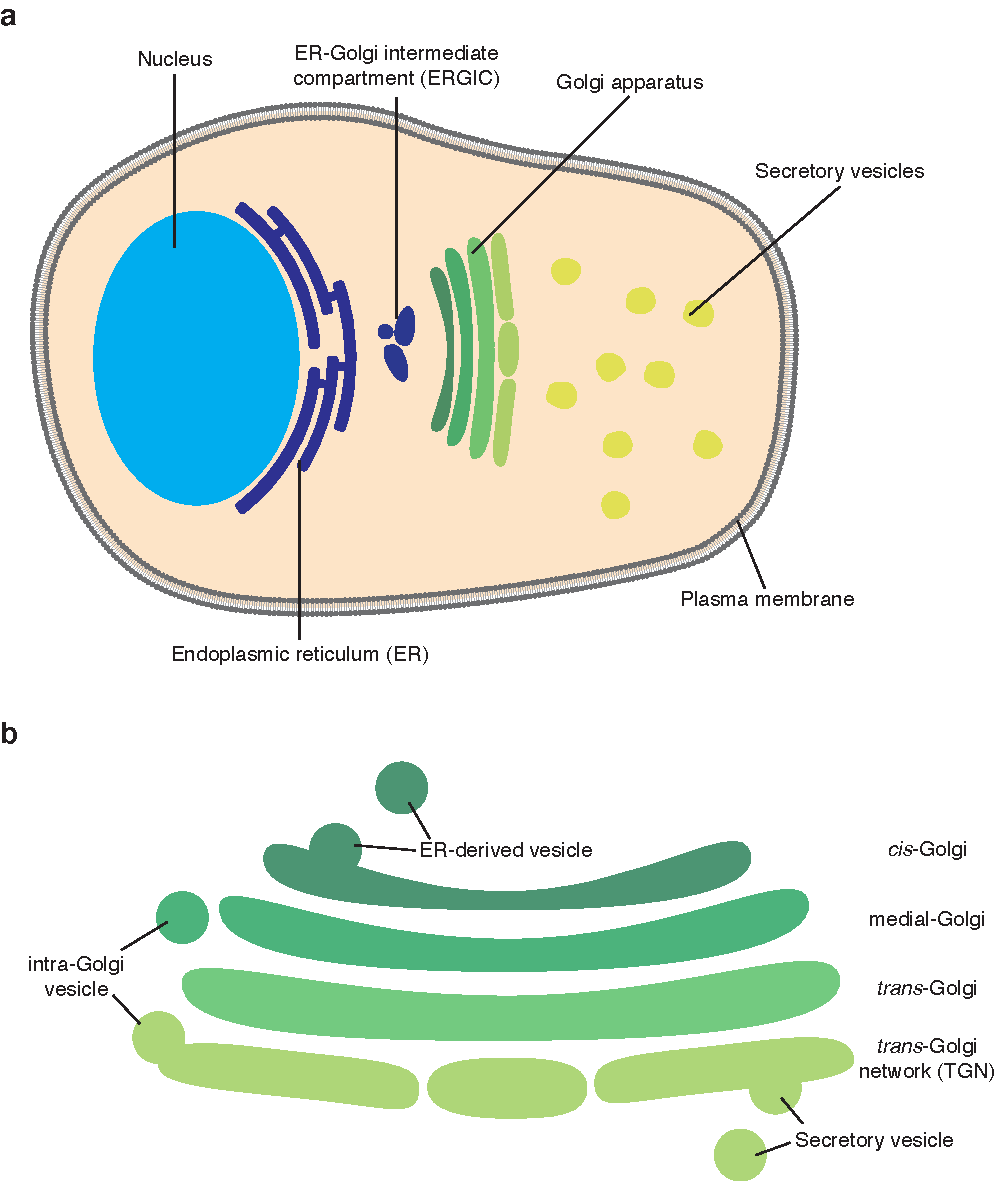
\includegraphics[keepaspectratio=true,width=\textwidth,height=\textheight]{chapters/chapter1/chapter1_Figure1.pdf}
    \caption{\textbf{(a)} Schematic overview of the mammalian secretory pathway. \textbf{(b)} Closer view of the mammalian Golgi apparatus. ER-derived vesicles arrive at the \emph{cis}-face of the Golgi, while secretory vesicles depart from the \emph{trans}-face. Cargo is exchanged between cisternae via intra-Golgi transport vesicles.}
    \label{fig:ch1fig1}
\end{figure}

In human cells, new proteins are translated from DNA-derived mRNA and co-translationally inserted into the rough ER. Within the lumen of the ER, proteins are folded and an initial quality control step is performed. This ensures that only properly folded proteins can exit the ER and continue their journey through the secretory pathway\cite{hetz_unfolded_2012}. Newly synthesized proteins are then packaged and transported in vesicles to the Golgi where they can be further modified and sorted to their correct destination (Figure~\ref{fig:ch1fig1}b). One driver in this sorting process is the decrease of pH (acidification) of the Golgi lumen from \emph{cis} (pH 6.7) to \emph{trans} (pH 6.0). pH differences are important for the acceptance and release of cargo from cargo adapters due to conformational changes and pH-dependent binding affinity\cite{brauer_structural_2019,wilson_ph-dependent_1993,ghosh_mannose_2003,olson_allosteric_2020}. Therefore, pH is of critical importance for the correct maintenance of Golgi cisterna identity\cite{linders_sugary_2020,fisher_bridging_2016,rivinoja_elevated_2009,maeda_chapter_2010}, as well as for the optimal function of glycosylation enzymes\cite{gawlitzek_ammonium_2000}.

After the newly synthesized proteins have sufficiently been modified, they are ready to be sorted at the TGN and exit the Golgi\cite{guo_protein_2014}. This final sorting step sends the newly synthesized proteins to their final location, including endosomes, lysosomes, the plasma membrane, and the extracellular space.


\section{Glycosylation}

One of the most important functions of the Golgi apparatus is to ensure the correct glycosylation of newly synthesized proteins. In vertebrates, glycosylation is a sequential process involving both the addition and trimming of glycan structures by glycosyltransferases and glycosidases\cite{lombard_carbohydrate-active_2014}. In contrast to other essential protein synthesis processes such as translation and transcription, glycosylation is not template-based (cf., DNA serves as a template for transcription and mRNA as a template for translation)\cite{gabius_sugar_2018}. Around 700 proteins are responsible for the full spectrum of around 7,000 unique glycan structures. Only ten different monosaccharides, fucose (Fuc), galactose (Gal), glucose (Glc), \emph{N}-acetylgalactosamine (GalNAc), \emph{N}-acetylglucosamine (GlcNAc), glucuronic acid (GlcA), mannose (Man), sialic acid (SA, also known as neuraminic acid), xylose (Xyl), and recently identified ribitol, are the necessary building blocks for glycans of mammalian cells\cite{cummings_repertoire_2009,joshi_glycosyltransferase_2018,nairn_handbook_2009,nairn_regulation_2008,narimatsu_atlas_2019,riemersma_human_2015}. Based on which amino acid residue of the protein the glycan is attached, O- and N-linked glycosylation can be distinguished. O-linked glycosylation occurs on the side chain hydroxyl oxygen of either serine or threonine residues, while N-linked glycosylation occurs on asparagine residues. As the work in this thesis is mainly focused on N-linked glycosylation, below I will shortly summarize the basic mechanism of N-linked glycosylation.

N-linked glycosylation begins in the ER where a precursor glycan consisting of 14 monosaccharides is transferred from the carrier lipid dolichol to the newly synthesized protein. Concurrent with translation, the precursor glycan is removed from dolichol and placed on N-linked glycosylation acceptor peptide sequons (Asn – X – (Ser/Thr)) of nascent polypeptides by oligosaccharyltransferase (OST)\cite{kornfeld_assembly_1985,lizak_x-ray_2011,ruiz-canada_cotranslational_2009,kelleher_evolving_2006,schreiner_novel_1994,valliere-douglass_glutamine-linked_2010,zielinska_precision_2010}. Before Golgi entry of the newly synthesized glycoproteins, distal glucose moieties are trimmed as an important step in the control of misfolded glycoproteins in the ER\cite{moremen_vertebrate_2012,helenius_roles_2004,lederkremer_glycoprotein_2009}. Once quality control is complete, the newly synthesized glycoproteins are transported to the Golgi, where the glycan structures are further trimmed, extended, and branched until the final form of the glycan is reached (Figure~\ref{fig:ch1fig2}, adapted from Figure 9.4 of \emph{Essentials of Glycobiology}\cite{varki_essentials_2017}).

\begin{figure}
    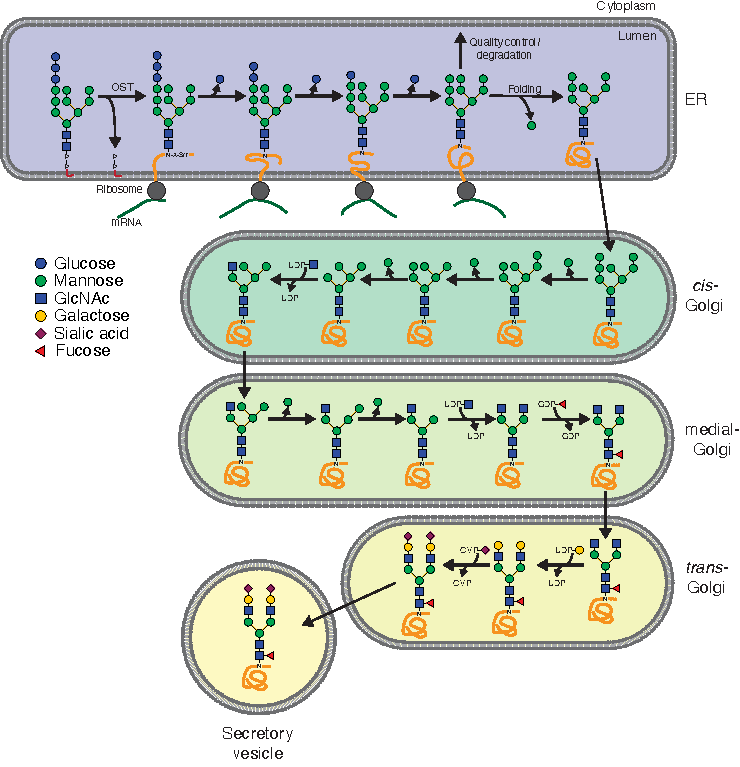
\includegraphics[keepaspectratio=true,width=\textwidth,height=\textheight]{chapters/chapter1/chapter1_Figure2.pdf}
    \caption{\textbf{The procesing and maturation of a biantennary, fucosylated N-glycan.} The immature glycan structure is transferred from dolichol phosphate to the nascent polypeptide in the ER. Following quality control, the folded glycoprotein is then exported to the Golgi where the final glycan structure is produced.}
    \label{fig:ch1fig2}
\end{figure}

The non-template-driven characteristics of glycosylation imply that stringent regulation of all glycosylation machinery is required to maintain physiological glycosylation. As such, small abnormalities can have a large effect on the final glycan product\cite{jaiman_golgi_2020} and currently already over 100 monogenic diseases have been found that are characterized by incorrect glycosylation. Collectively, these diseases are known as congenital disorders of glycosylation (CDG)\cite{linders_sugary_2020,fisher_bridging_2016,freeze_genetic_2006,freeze_solving_2014}. Therefore, the proper localization of all glycosylation machinery and other required factors is paramount.


\section{Membrane Fusion}

Crucial to all transport steps in mammalian cells is the delivery of (cargo) proteins from one organelle, or organellar sub-compartment, to the next. Considering the compartmentalization of the secretory pathway, the prevailing theory of protein transport in mammalian cells is via membrane vesicles. Once a vesicle has been released and is destined for an organelle, such as the Golgi apparatus, the vesicle must fuse its membrane with the membrane of the accepting compartment to transfer the cargo to the intraorganellar lumen. This step is mediated by SNARE proteins.

SNAREs (soluble \emph{N}-ethylmaleimide-sensitive factor attachment protein (SNAP) receptors) mediate all fusion events in eukaryotic cells, except for mitochondrial fusion\cite{jahn_snares_2006,hong_snares_2005}. The human SNARE family consists of 36 members, which all carry one or two SNARE motifs, domains of approximately 60-70 amino acid residues arranged in heptad repeats\cite{weimbs_conserved_1997}. Most SNAREs are anchored to the membrane and most SNAREs contain a transmembrane domain, while others can be anchored through lipid modifications such as palmitoylation or prenylation.

Mammalian SNAREs can be roughly classified into two groups based on their membrane location: the vesicular SNAREs (v-SNARE) present on cargo vesicles and target SNAREs (t-SNARE) on the acceptor membrane. In some cases, this classification can be inconsistent, for instance when SNAREs are involved in bidirectional (anterograde and retrograde) transport of molecules or homotypic vesicle fusion without defined donor or acceptor compartments. SNAREs can also be classified by the central functional residue in the SNARE motif: R-SNAREs contain an arginine residue while Q-SNAREs (these can be subdivided in Qa, Qb, Qc or, Qbc depending on their location in the SNARE bundle) contain a glutamine residue55. For successful membrane fusion, four SNARE motifs, one R-SNARE and 3 Q-SNAREs, interact together to form a tight coiled-coil bundle that brings the vesicular and acceptor membranes together (Figure~\ref{fig:ch1fig3}). This mechanism overcomes the energy barrier of membrane fusion.

\begin{figure}
    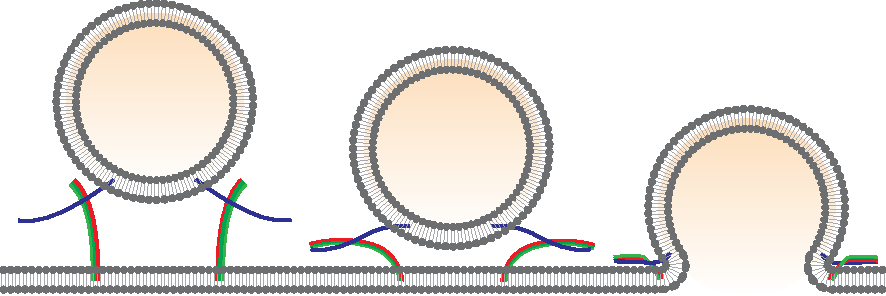
\includegraphics[keepaspectratio=true,width=\textwidth,height=\textheight]{chapters/chapter1/chapter1_Figure3.pdf}
    \caption{\textbf{SNARE-mediated membrane fusion at the ER - Golgi interface.} The t-SNARE complex on the acceptor membrane (red: Qa-SNARE, green: Qb/R-SNARE) and the v-SNARE (blue: Qc-SNARE) on the vesicular membrane come into close proximity and form a \emph{trans}-SNARE complex. As this complex tightens, the two membranes are forced closer to each other and the lipid bilayers fuse.}
    \label{fig:ch1fig3}
\end{figure}

Considering the Golgi as the central hub of the mammalian cell, it is an important location where many membrane fusion events occur. Vesicles containing newly synthesized proteins from the ER, vesicles going to and from the plasma membrane, and vesicles involved in intra-Golgi trafficking all need to fuse with Golgi membranes. Two main models of Golgi apparatus transport exist. The first model is the vesicular trafficking model, where each cisterna is a static sub-compartment and cargo molecules are transported by vesicles between the cisternae\cite{cottam_retrograde_2012}. The second, more widely-accepted model is cisternal maturation in which vesicles with newly synthesized proteins from the ER fuse with each other to form the \emph{cis}-Golgi. Each cisterna is highly dynamic and gradually matures into \emph{trans}-Golgi through accepting lipids and glycosylation enzymes from later Golgi cisternae\cite{cottam_retrograde_2012}. At the ER – Golgi trafficking interface in the cisternal maturation model, four distinct trafficking steps can be identified: anterograde transport from ER to the ER – Golgi intermediate compartment (ERGIC), from ERGIC to \emph{cis}-Golgi, intra-Golgi transport between cisternae and retrograde trafficking from \emph{cis}-Golgi to the ER. In these four different trafficking steps, syntaxin-5 (Stx5) is the most important Qa-SNARE, participating in three out of the four different SNARE complexes\cite{linders_stx5-mediated_2019} (Figure~\ref{fig:ch1fig4}). The formation of different SNARE complexes with unique cognate SNAREs is beneficial to the specificity of membrane trafficking, ensuring that the right cargo is transported to the right destination.

\begin{figure}
    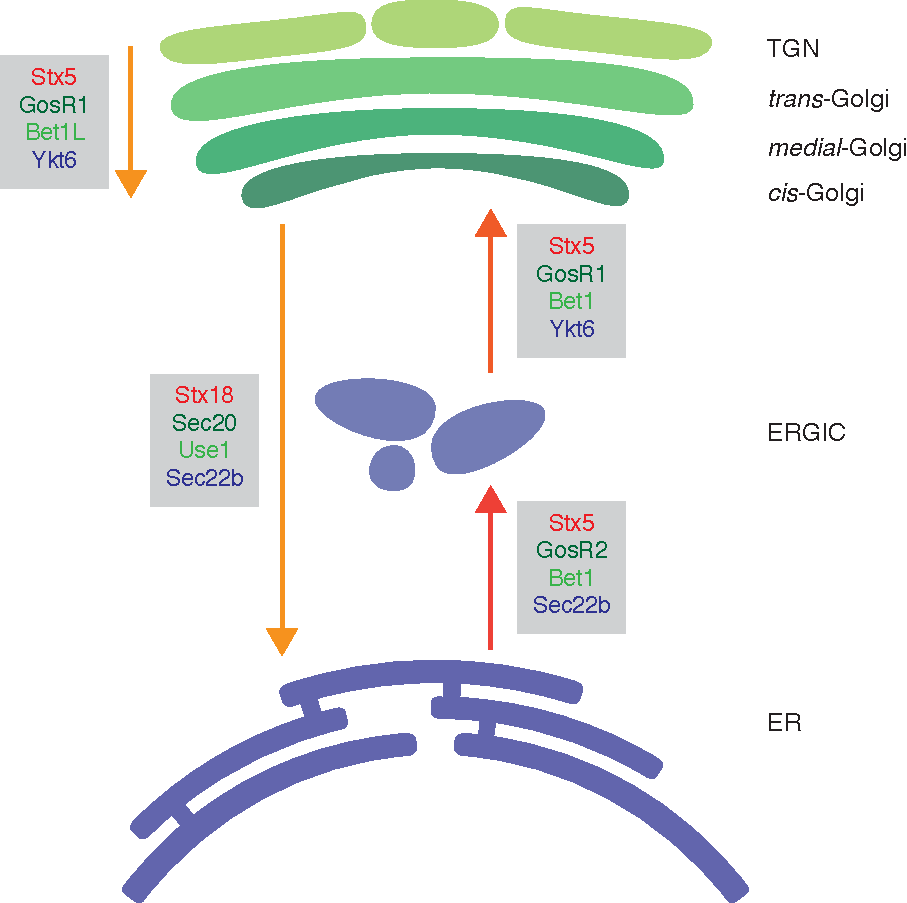
\includegraphics[keepaspectratio=true,width=\textwidth,height=\textheight]{chapters/chapter1/chapter1_Figure4.pdf}
    \caption{\textbf{Schematic overview of SNARE complexes at the ER-Golgi interface in mammalian cells.} Adapted from Chapter 5, Figure~\ref{fig:ch5fig1}.}
    \label{fig:ch1fig4}
\end{figure}

\vspace{\baselineskip}

Taken together, the secretory pathway is the veritable heart of the eukaryotic cell, by ensuring that newly synthesized proteins are delivered in the correct composition and at the correct location. Each transport step is finely tuned for optimal performance and maximum fidelity of the respective cargo. Unfortunately, only small abnormalities in this trafficking system can cause large problems on both the cellular and organism level, but the molecular mechanisms are often poorly understood. In this thesis, I addressed the molecular mechanisms behind CDGs of components involved in protein transport from ER to Golgi.

\clearpage

\section{Scope of this Thesis}

The principal aim of this thesis is to obtain a better understanding of the involvement of intracellular trafficking proteins in ER-Golgi transport and glycosylation. To achieve this, I performed cell biological and biochemical experiments to uncover the molecular mechanism of patients with novel CDGs.

\textbf{Chapter 2} provides an overview of all CDGs that are related to intracellular trafficking proteins. Recent developments in diagnostic methods for CDG have enabled the discovery of new genetic variants in trafficking proteins that result in glycosylation disorders. I discuss these developments and how they help understand ER-Golgi trafficking better. In \textbf{chapter 3}, I demonstrate a newly developed technique based on fluorescence lifetime imaging microscopy (FLIM) to measure intraorganellar pH with high accuracy. I apply the technique on both static organelle markers and dynamic cargo proteins. This improved imaging technique is subsequently applied in \textbf{chapter 4} to determine the role of V-ATPase assembly factor TMEM199 in ER-Golgi transport and luminal acidification.

An integral component of ER-Golgi transport, syntaxin-5, is the focus of the second part of this thesis. \textbf{Chapter 5} provides a comprehensive examination of all published literature on syntaxin-5 and disseminates the differences and similarities of syntaxin-5 and ER-Golgi trafficking in both mammals and yeast. This forms the preface to \textbf{chapter 6}, where I present the discovery of a new genetic variant in syntaxin-5 resulting in a CDG with a severe phenotype. I demonstrate the molecular mechanism behind this CDG and thereby improve our understanding of the role of syntaxin-5 in mammalian intracellular trafficking and glycosylation.

